\chapter{\ifproject%
% \ifenglish Experimentation and Results\else การทดลองและผลลัพธ์\fi
% \else%
\ifenglish System Evaluation\else การประเมินระบบ\fi
\fi}

เนื่องจากนักสังคมสงเคราะห์ที่ปฏิบัติงานในโรงพยาบาลมหาราชนครเชียงใหม่ยังไม่มีระบบที่สามารถรองรับการทำงานได้อย่างมีประสิทธิภาพเพียงพอ หากต้องรอให้ระบบที่พัฒนาขึ้นเสร็จสมบูรณ์ อาจใช้ระยะเวลาหลายเดือน

เพื่อแก้ไขปัญหาในระยะเริ่มต้น ทางคณะผู้จัดทำโครงงานได้วางแนวทางในการให้ความช่วยเหลือเบื้องต้นแก่เจ้าหน้าที่นักสังคมสงเคราะห์ ควบคู่ไปกับการสร้างต้นแบบของแบบฟอร์มบันทึกข้อมูลเบื้องต้น เพื่อศึกษาประเด็นปัญหาที่อาจเกิดขึ้นในการพัฒนาและนำไปสู่การปรับปรุงแนวทางการทำงานใน Sprint 1 อย่างมีประสิทธิภาพ

\section{การทดลองขึ้นหน้าเว็บแอปพลิเคชัน}

โดยจะเป็นการทดลองขึ้นหน้าแบบฟอร์มกรอกประวัติผู้ป่วย ในหน้าแรกจะเป็นการกรอกข้อมูลส่วนตัวของผู้ป่วย โดยจะมีข้อมูลบางชนิดที่ต้องทำเป็น Drop-down box เพื่อลดความผิดพลาดจากการพิมพ์ของนักสังคมสงเคราะห์ และต้องกรอกให้สมบูรณ์จึงจะสามารถกรอกหน้าต่อไปได้

\begin{figure}[H]
    \begin{center}
        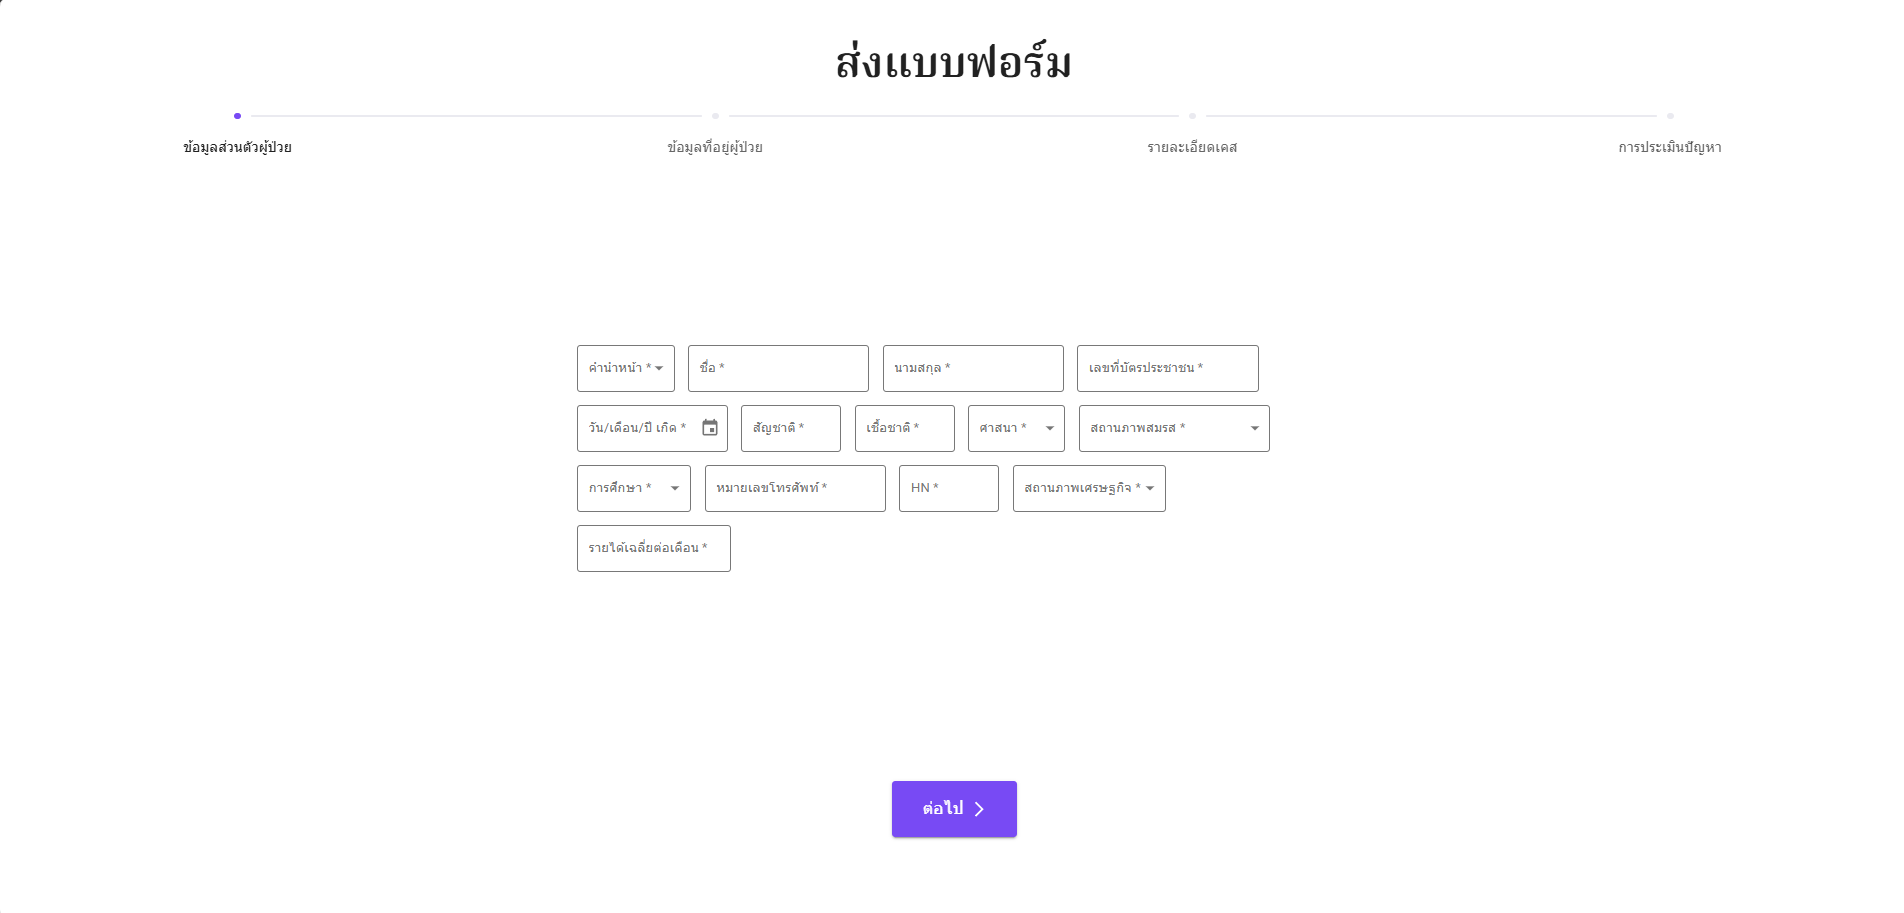
\includegraphics[width=1\textwidth]{Screenshot 2025-03-06 200233.png}
    \end{center}
    \caption[หน้ากรอกข้อมูลส่วนตัวผู้ป่วย]{หน้ากรอกข้อมูลส่วนตัวผู้ป่วย}
\end{figure}
\newpage
หน้าต่อมาคือหน้าที่ใช้กรอกที่อยู่ของผู้ป่วย ซึ่งจะสามารถกรอกได้ 2 รูปแบบ คือ
\begin{enumerate}
    \item กรอกจังหวัด อำเภอ และตำบลจากนั้นรหัสไปรษณีย์จะ Auto-complete ให้เอง
    \item กรอกแค่หมายเลขไปรษณีย์แล้ว จังหวัด อำเภอ และตำบลจะ Auto-complete ให้เอง 
\end{enumerate}
\begin{figure}[H]
    \begin{center}
        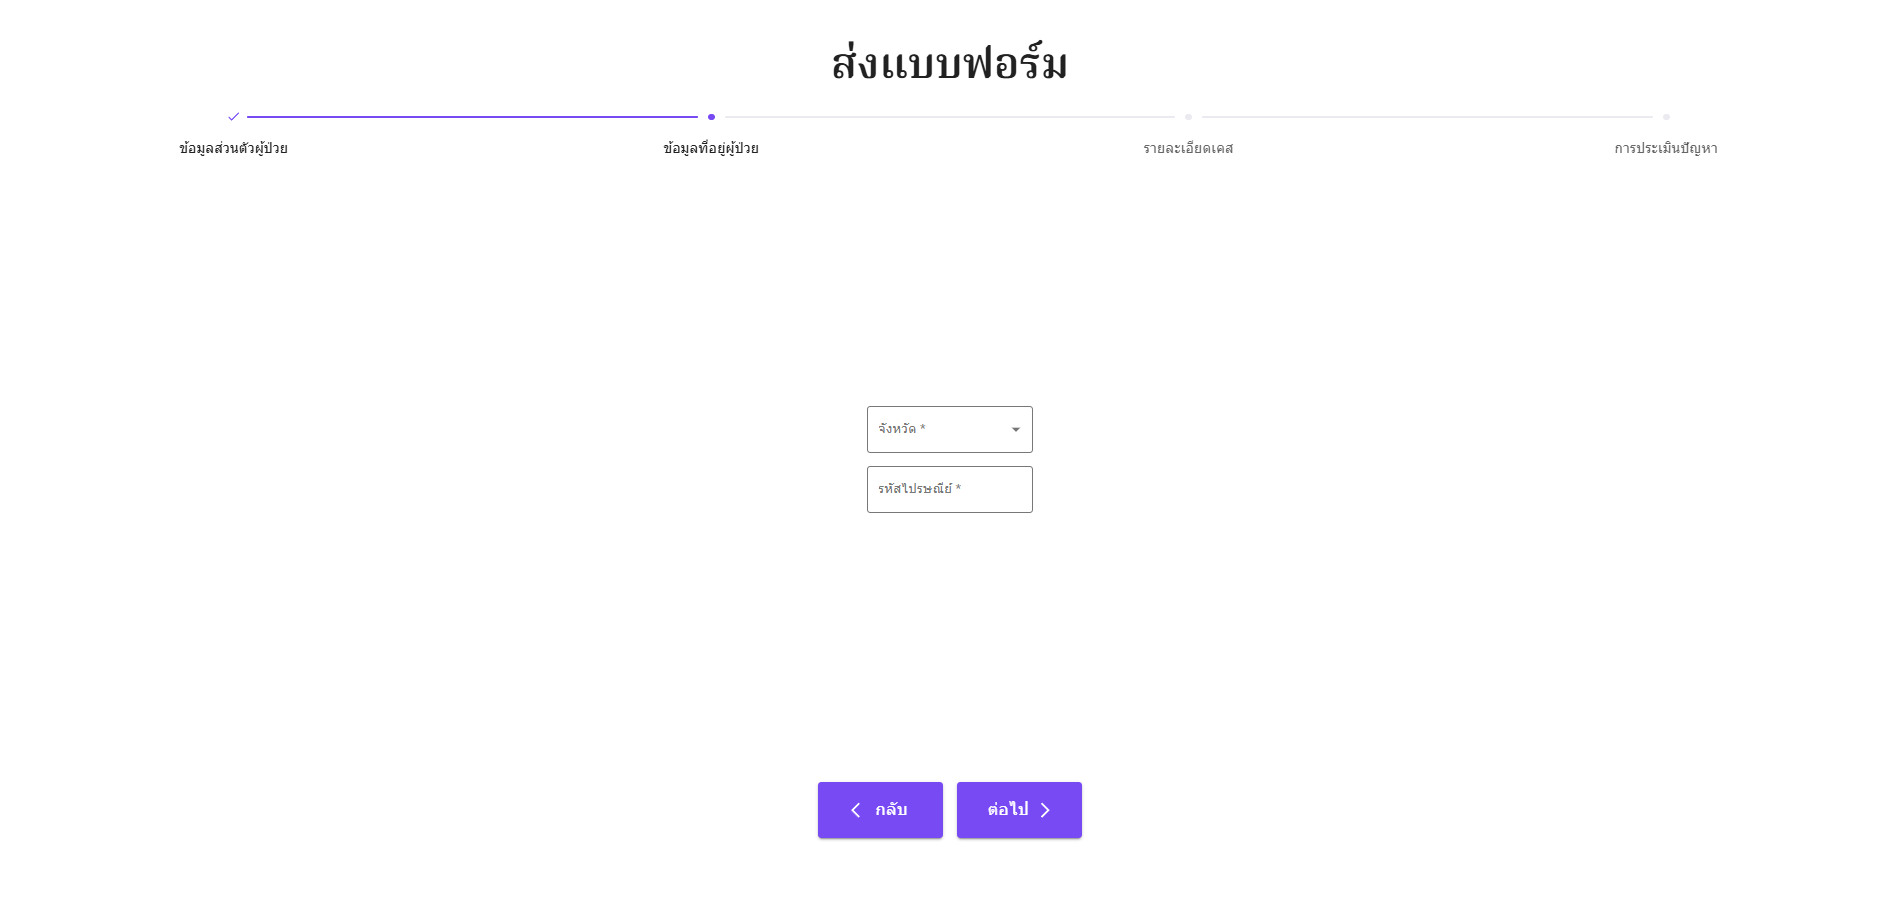
\includegraphics[width=1\textwidth]{Screenshot 2025-03-06 200323.png}
    \end{center}
    \caption[หน้ากรอกที่อยู่ผู้ป่วย]{หน้ากรอกที่อยู่ผู้ป่วย}
\end{figure}

\section{ความช่วยเหลือในเบื้องต้น}

ทางคณะผู้จัดทำโครงงาน ได้ทดลองใช้ Microsoft Form ร่วมกับ Microsoft Onedrive และ Microsoft Power Automate เพื่อให้สามารถเก็บข้อมูลและเข้าถึงข้อมูลผู้ป่วย โดยที่คอมพิวเตอร์ทุกเครื่องที่กำหนดสามารถที่จะเข้าถึงไฟล์ได้โดยตรง โดยเมื่อนักสังคมสงเคราะห์กรอกข้อมูลผู้ป่วยลงใน Mircosoft Form ทาง Microsoft Power Automate จะทำการสร้างโฟลเดอร์ของผู้ป่วยแต่ละคนใน Onedrive หากผู้ป่วยคนนั้นยังไม่มีโฟลเดอร์ของตนเอง และนำข้อมูลที่กรอกไว้ ใส่ลงในโฟลเดอร์นั้น

แต่เนื่องจาก Onedrive มีพื้นที่ที่ใช้ได้อย่างจำกัด (15 GB) ทำให้ไม่สามารถจัดเก็บข้อมูลผู้ป่วยได้อย่างเพียงพอ จึงไม่ได้นำวิธีการนี้ไปใช้จริง